%\documentclass[conference,final]{IEEEtran}
%\documentclass{acm_proc_article-sp}

\documentclass{sig-alternate}

%\documentclass{acm_proc_article-sp}

\usepackage[numbers, sort, compress]{natbib}
\usepackage{graphicx}
\usepackage{amsmath}
\usepackage{amssymb}
\usepackage{color}
\usepackage{ifpdf}

\usepackage{dcolumn}
\usepackage{float}
\usepackage[utf8]{inputenc}
\usepackage{multirow}
\usepackage{rotating}

\usepackage[tight]{subfigure}



%\usepackage[numbers, sort, compress]{natbib}
%\usepackage{latex8}
%\usepackage{float}
%\usepackage{times}    
\usepackage{url}
\usepackage{listings}   
\usepackage{paralist}    
\usepackage{wrapfig}    
%\usepackage[small,it]{caption}
\usepackage{multirow}
\usepackage{ifpdf}
%\usepackage{srcltx}
%\usepackage{subfigure}
\usepackage{xspace}
\usepackage{keyval}  
\usepackage{color}

\definecolor{listinggray}{gray}{0.95}
\definecolor{darkgray}{gray}{0.7}
\definecolor{commentgreen}{rgb}{0, 0.4, 0}
\definecolor{darkblue}{rgb}{0, 0, 0.4}
\definecolor{middleblue}{rgb}{0, 0, 0.7}
\definecolor{darkred}{rgb}{0.4, 0, 0}
\definecolor{brown}{rgb}{0.5, 0.5, 0}

\usepackage[normalem]{ulem}
\makeatletter
\def\cyanuwave{\bgroup \markoverwith{\lower3.5\p@\hbox{\sixly \textcolor{cyan}{\char58}}}\ULon}
\def\reduwave{\bgroup \markoverwith{\lower3.5\p@\hbox{\sixly \textcolor{red}{\char58}}}\ULon}
\def\blueuwave{\bgroup \markoverwith{\lower3.5\p@\hbox{\sixly \textcolor{blue}{\char58}}}\ULon}
\font\sixly=lasy6 % does not re-load if already loaded, so no memory problem.
\makeatother


\begin{document}
%\conferenceinfo{WOODSTOCK}{'97 El Paso, Texas USA}
% \conferenceinfo{ECMLS'11,} {June 8, 2011, San Jose, California, USA.}
% \CopyrightYear{2011}
% \crdata{978-1-4503-0702-4/11/06}
% \clubpenalty=10000
% \widowpenalty = 10000

%!TEX root = sc12/pstar-sc2012-ieee.tex
\newif\ifdraft
%\drafttrue
\ifdraft
\newcommand{\onote}[1]{ {\textcolor{cyan} { (***Ole: #1) }}}
\newcommand{\terminology}[1]{ {\textcolor{red} {(Terminology used: \textbf{#1}) }}}
\newcommand{\owave}[1]{ {\cyanuwave{#1}}}
\newcommand{\jwave}[1]{ {\reduwave{#1}}}
\newcommand{\alwave}[1]{ {\blueuwave{#1}}}
\newcommand{\jhanote}[1]{ {\textcolor{red} { ***shantenu: #1 }}}
\newcommand{\alnote}[1]{ {\textcolor{blue} { ***andreL: #1 }}}
\newcommand{\amnote}[1]{ {\textcolor{blue} { ***andreM: #1 }}}
\newcommand{\smnote}[1]{ {\textcolor{brown} { ***sharath: #1 }}}
\newcommand{\msnote}[1]{ {\textcolor{cyan} { ***mark: #1 }}}
\newcommand{\note}[1]{ {\textcolor{magenta} { ***Note: #1 }}}
\else
\newcommand{\onote}[1]{}
\newcommand{\terminology}[1]{}
\newcommand{\owave}[1]{#1}
\newcommand{\jwave}[1]{#1}
\newcommand{\alnote}[1]{}
\newcommand{\amnote}[1]{}
\newcommand{\athotanote}[1]{}
\newcommand{\smnote}[1]{}
\newcommand{\jhanote}[1]{}
\newcommand{\msnote}[1]{}
\newcommand{\note}[1]{}
\fi

\newcommand{\pilot}{Pilot\xspace}
\newcommand{\pilots}{Pilots\xspace}
\newcommand{\pilotjob}{Pilot-Job\xspace}
\newcommand{\pilotjobs}{Pilot-Jobs\xspace}
\newcommand{\computeunit}{Compute Unit\xspace}
\newcommand{\computeunits}{Compute Units\xspace}
\newcommand{\cu}{CU\xspace}
\newcommand{\cus}{CUs\xspace}
\newcommand{\cs}{Compute Service\xspace}
\newcommand{\css}{Compute Services\xspace}
\newcommand{\pcs}{Pilot Compute Service\xspace}
\newcommand{\dataunit}{Data Unit\xspace}
\newcommand{\dataunits}{Data Unit\xspace}
\newcommand{\du}{DU\xspace}
\newcommand{\dus}{DUs\xspace}
\newcommand{\pilotdata}{Pilot-Data\xspace}
\newcommand{\pd}{PD\xspace}
\newcommand{\pds}{Pilot Data Service\xspace}
\newcommand{\pdss}{Pilot Data Services\xspace}
\newcommand{\su}{SU\xspace}
\newcommand{\sus}{SUs\xspace}
\newcommand{\schedulableunit}{Schedulable Unit\xspace}
\newcommand{\schedulableunits}{Schedulable Units\xspace}
\newcommand{\cc}{c\&c\xspace}
\newcommand{\CC}{C\&C\xspace}

\lstdefinestyle{myListing}{
  frame=single,   
  backgroundcolor=\color{listinggray},  
  %float=t,
  language=C,       
  basicstyle=\ttfamily \footnotesize,
  breakautoindent=true,
  breaklines=true
  tabsize=2,
  captionpos=b,  
  aboveskip=0em,
  belowskip=-2em,
  %numbers=left, 
  %numberstyle=\tiny
}      

\lstdefinestyle{myPythonListing}{
  frame=single,   
  backgroundcolor=\color{listinggray},  
  %float=t,
  language=Python,       
  basicstyle=\ttfamily \footnotesize,
  breakautoindent=true,
  breaklines=true
  tabsize=2,
  captionpos=b,  
  %numbers=left, 
  %numberstyle=\tiny
}

\newcommand{\up}{\vspace*{-1em}}
\newcommand{\upp}{\vspace*{-0.5em}}
\newcommand{\numrep}{8 }
\newcommand{\samplenum}{4 }
\newcommand{\tmax}{$T_{max}$ }
\newcommand{\tc}{$T_{C}$ }
\newcommand{\tcnsp}{$T_{C}$}
\newcommand{\bj}{BigJob}

%  \setlength{\parskip}{0.05ex} % 1ex plus 0.5ex minus 0.2ex}
%  \setlength{\parsep}{0pt}
%  %\setlength{\headsep}{0pt}
%  \setlength{\topskip}{0pt}
%  \setlength{\topmargin}{0pt}
%  %\setlength{\topsep}{0pt}
%  \setlength{\partopsep}{0pt}

% This is now the recommended way for checking for PDFLaTeX:


\ifpdf
\DeclareGraphicsExtensions{.pdf, .jpg, .tif}
\else
\DeclareGraphicsExtensions{.eps, .jpg}
\fi

\tolerance=1000
\hyphenpenalty=10


% \author{
%   Andre Luckow$^{1}$, Mark Santcroos$^{2,1}$, Ole Weidner$^{1}$, Andre Merzky$^{1}$, Sharath Maddineni$^{1}$, Shantenu Jha$^{3,1*}$\\[0.5em]
%   \small{\emph{$^{1}$Center for Computation \& Technology, Louisiana State University, USA}}\\[-0.3em]
%   \small{\emph{$^{2}$Bioinformatics Laboratory, Academic Medical Center, University of Amsterdam, The Netherlands}}\\[-0.3em]
%   \small{\emph{$^{3}$ Rutgers University, Piscataway, NJ 08854, USA}}\\[-0.3em]
% %  \small{\emph{$^{4}$ School of Informatics, University of Edinburgh, UK }}\\[-0.3em]
%   \small{\emph{$^{*}$Contact Author: \texttt{shantenu.jha@rutgers.edu}}}\\[-0.3em]
%   \up\up\up }


\title{P*: A Model of Pilot-Abstractions\up}
\numberofauthors{5}
\author{
\alignauthor Andre Luckow\\
       \affaddr{Center for Computation\newline and Technology}\\
       \affaddr{Louisiana State University}\\
       \affaddr{216 Johnston}\\
       \affaddr{Baton Rouge, LA} \\
       \email{aluckow@cct.lsu.edu}
\and
\alignauthor Mark Santcroos\\
       \affaddr{Bioinformatics Laboratory}\\
       \affaddr{Academic Medical Center}\\
       \affaddr{University of Amsterdam}\\
       \affaddr{Meibergdreef 9}\\
       \affaddr{Amsterdam, The Netherlands}
       \email{m.a.santcroos@amc.uva.nl}
\and
\alignauthor Ole Weidner\\
       \affaddr{Center for Computation\newline and Technology}\\
       \affaddr{Louisiana State University}\\
       \affaddr{216 Johnston}\\
       \affaddr{Baton Rouge, LA}
       \email{oweidner@cct.lsu.edu}
\and
\alignauthor Andre Merzky\\
       \affaddr{Center for Computation\newline and Technology}\\
       \affaddr{Louisiana State University}\\
       \affaddr{216 Johnston}\\
       \affaddr{Baton Rouge, LA}
       \email{amerzky@cct.lsu.edu}
\alignauthor Sharath Maddineni\\
       \affaddr{Center for Computation\newline and Technology}\\
       \affaddr{Louisiana State University}\\
       \affaddr{216 Johnston}\\
       \affaddr{Baton Rouge, LA}
       \email{smaddineni@cct.lsu.edu}
\and
\alignauthor Shantenu Jha\titlenote{Author for correspondence}\\
      \affaddr{Center for Autonomic Computing}\\
     \affaddr{Rutgers University}\\
      \affaddr{94 Brett Road}\\
      \affaddr{Piscataway, NJ}
     \email{shantenu.jha@rutgers.edu}
}

\date{}

\maketitle

\begin{abstract} 
 % Distributed cyberinfrastructures (CI) and applications require the
  % ability to determine and utilize resource
  % selection\alnote{selection somehow does not fit} at runtime
  % (dynamically), and not just before execution (statically).
  \pilotjobs support effective distributed resource utilization, and 
  are arguably one of the most widely-used distributed
  computing abstractions,
  % they have been utilized on many production distributed
  % cyberinfrastructures.  they have been notable in their ability to
  %\alnote{the following sentence is just a fragement}
  as measured by the number and types of applications that use them,
  as well as the number of production distributed cyberinfrastructures
  that support them.  Not surprisingly, there are multiple, distinct
  and incompatible implementations of pilot-jobs. Often these
  implementations are strongly coupled to the distributed
  cyberinfrastructure they were originally designed for.
  Additionally, in spite of broad uptake, there does not exist a well
  defined, unifying conceptual model of \pilotjobs which can be used
  to define, compare and contrast different implementations. This
  presents a barrier to extensibility and interoperability. This paper
  is an attempt to (i) provide a minimal but complete model (P*) of
  \pilotjobs, (ii) establish the generality of the P* Model by mapping
  various existing and well known \pilotjob frameworks such as Condor
  and DIANE to P*, (iii) derive an interoperable and extensible API
  for the P* Model (Pilot-API), (iv) validate the implementation of
  the Pilot-API by concurrently using multiple {\it distinct}
  pilot-job frameworks on distinct production distributed
  cyberinfrastructures, and (v) apply the P* Model to \pilotdata.
\end{abstract}
%\category{H.4}{Information Systems Applications}{Miscellaneous}
%terms{Theory}
%\keywords{ACM proceedings, \LaTeX, text tagging}
%\up\up

\section{Introduction and Overview} 

The seamless uptake of distributed infrastructures by scientific
applications has been limited by the availability of extensible,
pervasive and simple-to-use abstractions at multiple levels -- at
development, deployment and execution stages of scientific
applications~\cite{dpagrid2009}.  Even where meaningful abstractions
exist, the challenges of providing them in an extensible, reliable and
scalable manner so as to support multiple applications and are
usable on different infrastructures are formidable.  The lack of
appropriate implementations has in fact resulted in ``one-off''
solutions that address challenges in a highly customized manner.
Tools and implementations are often highly dependent on and tuned to a
specific execution environment, further impacting portability,
reusability and extensibility.  Semantic and interface incompatibility
are certainly barriers, but so is the lack of a common architecture
and conceptual framework upon which to develop similar tools a
barrier.

%reinforces the fragmentation~\cite{dpa_surveypaper}.
% there remains, scope for improvement in both the range and number of
% supported abstractions and the type of infrastructure over which such
% abstractions are made available.

This general state of affairs also captures the specific state of the
abstractions provided by {\it \pilotjobs (PJ)}. \pilotjobs have been
one of the most successful abstractions in distributed
computing. Distributed cyber/e-infrastructure is by definition
comprised of a set of resources that is fluctuating -- growing,
shrinking, changing in load and capability (in contrast to a static
resource utilization model of traditional parallel
and cluster computing systems).  The ability to utilize a dynamic resource
pool is thus an important attribute of any application that needs to
utilize distributed cyberinfrastructure (DCI) efficiently. As a
consequence of providing a simple approach for decoupling workload
management and resource assignment/scheduling, PJ provide an
effective abstraction for dynamic execution and resource utilization in
a distributed context.


The fundamental reason for the success of the PJ abstraction is that
PJ liberate applications/users from the challenging requirement of
mapping specific tasks onto explicit heterogeneous and dynamic
resource pools.  PJ also thus shields application from having to
load-balance tasks across such resources.  The \pilotjob abstraction
is also a promising route to address specific requirements of
distributed scientific applications, such as coupled-execution and
application-level scheduling~\cite{ko-efficient,DBLP:conf/hpdc/KimHMAJ10}.


A variety of PJ frameworks have emerged:
Condor-G/ Glide-in~\cite{condor-g}, Swift~\cite{Wilde2011},
DIANE~\cite{Moscicki:908910}, DIRAC~\cite{1742-6596-219-6-062049},
PanDA~\cite{1742-6596-219-6-062041}, ToPoS~\cite{topos},
Nimrod/G~\cite{10.1109/HPC.2000.846563}, Falkon~\cite{1362680} and
MyCluster~\cite{1652061} to name a few. Although they are all, for the
most parts, functionally equivalent -- they support the decoupling of
workload submission from resource assignment -- it is often impossible
to use them interoperably or even just to compare them functionally or
qualitatively.  The situation is reminiscent of the proliferation of
functionally similar yet incompatible workflow systems, where in spite
of significant a posteriori effort on workflow system extensibility
and interoperability (thus providing post-facto justification of its
needs), these objectives remains difficult if not infeasible.

%Where effective abstractions exist a problem in the 
%The general problem applies to the specific situation of pilot-jobs.

%Different projects and users have rolled-out their own PJ
%abstractions.  

% The fact that users have voted with their feet for PJs reinforces that
% the PJ abstraction is both a useful and correct abstraction for
% distributed CI; 

% the fact that it has become an ``unregulated cottage
% industry'' reaffirms the lack of common nomenclature, integration,
% interoperability and extension, and poses barriers to extensibility and
% interoperability as a consequence. 


% Also, maybe interoperability isnt what is desired, but reusability
% and or ease of customisation.  Talk about analogy with workflow
% systems.  Interestingly there exist many implementations of the PJ
% abstraction, wherein d

% Interestingly there exist many implementations of the PJ abstraction,
% wherein different projects and users have rolled-out their own. The
% fact that users have voted with their feet for PJs reinforces that the
% Pilot-Job is both a useful and correct abstraction for distributed CI;
% the fact that it has become an ``unregulated cottage industry''
% reaffirms the lack of common nomenclature, integration,
% interoperability and extension.


% In \S{III} we introduce TROY -- A Tiered Resource OverlaY -- as an
% implementation of the P* Model. TROY provides an API for the P* Model
% and exposes the semantics of PJ frameworks; TROY also has a runtime
% system that enables it to work with different middleware on
% heterogeneous distributed platforms.

% Implementations of PJ frameworks, such as BigJob and DIANE, are
% integrated into TROY via an adaptor mechanism; we posit that the TROY
% framework and API can be used for most, if not all PJ frameworks.

% The P* Model captures the essence of most, if not all existing PJ
% frameworks.

We present the P* Model in \S\ref{sec:pilot-model}. Our objective is to provide
a minimal, but complete model -- hence referred to as P* Model, for \pilotjob
abstractions. The P* Model provides a conceptual basis to compare and contrast
different PJ frameworks -- which to the best of our knowledge is the first such
attempt. In \S\ref{sec:pilot-job-frameworks} we validate this claim by analyzing
well-known PJ frameworks (BigJob, Condor-G/Glide-in, DIANE, Swift-Coaster) using
the P* Model.

%Before validating this claim with empirical evidence

% \S{V} we present and validate

\S\ref{sec:pilot-api} of this paper motivates and describes the Pilot-API;  we
discuss how % BigJob, Condor-G/Glide-in~\cite{condor-g} and
% DIANE~\cite{Moscicki:908910} --
existing and widely used \pilotjob frameworks, can be used through the
Pilot-API.  \S\ref{sec:exp_res} describes the experiments and performance
measurements used to characterize the workings of the Pilot-API and to
demonstrate interoperability across middleware, platform and different
PJ frameworks.  To further substantiate the impact of P*, we will
demonstrate interoperability between different PJ frameworks -- BigJob
and DIANE. We believe this is also the first demonstration of
concurrent interoperation of different \pilotjob implementations.
Performance advantages arising from the ability to distribute part of a
data-intensive workload are discussed; interoperable capabilities
increase flexibility in resource selection and optimization.

% After validating the P* Model -- as measured by extensibility and
% interoperability -- 
We investigate generalizations to the base P* Model
in \S\ref{sec:pilot-data}.  A natural and logical extension of the
P* Model arises from the need to extend it to include data in
addition to computational tasks.  This leads to analogous abstraction
to the \pilotjob: the \emph{\pilotdata (PD)} abstraction.  The
potentially consistent treatment of data and compute suggests
symmetrical compute and data elements in the model; thus we refer
to this model as the P* Model ("P-star").

%Before discussing the P* Model, 

It is worth noting that \pilotjobs are used on every major
national and international DCI, including NSF/XSEDE,
NSF/DOE Open Science Grid, EU EGI and others, to support hundreds and
thousands of tasks daily, thus we believe the impact and validation of
this paper lies in its ability to not only influence but also bridge
the theory and practice of \pilotjobs, and thus multiple domains of
science dependent on distributed cyberinfrastructure.





%  which is also partly motivated by
% the status of the usage and availability of the pilot abstraction
% vis-\`{a}-vis the current landscape of distributed applications and
% cyberinfrastructure.

 % Collectively pilot-jobs support
% hundreds of thousands if not millions of tasks every day.  As we will
% show, the Pilot-API provides a single uniform API to PJ-frameworks
% thus providing for the first time... removing barriers to...
% \jhanote{fix..}


\section{The P* Model of Pilot-\\Abstractions}
\label{sec:pilot-model}


To provide a common analytical framework to understand the most
commonly used \pilotjobs, we present the P* Model of
pilot-abstractions. The P* model is derived from an analysis of many
\pilotjob implementations; based upon this analysis, we first present
the common {\it elements} of the P* Model, followed by a description
of the {\it characteristics} that determine the interaction of these
elements and the overall functioning of a \pilotjob framework that is
consistent with the P* Model.

%All pilot-job frameworks (whether they adhere rigorously to the P*
%model or not), have these {\it elements}, but differ in {\it
%  characteristics}.
%specific attributes \alnote{What would be an attribute in this
%  context?} and

% Further, we will show that
% these elements and interactions can be used to describe a pilot-data
% model.
 
Before we proceed to discuss the P* Model, it is important to
emphasize that there exist a plethora of terms --- abstraction, model,
framework, and implementation, that are overloaded and overlapping,
and often even used inconsistently in the literature; thus we
establish their context and usage in this paper.

\emph{Terms and Usage:} The \emph{ abstraction} of a \pilotjob
generalizes the reoccurring concept of utilizing a placeholder job as a
container for a set of compute tasks; instances of that placeholder
job are commonly referred to as \emph{\pilotjobs} or
\emph{pilots}. The P* \emph{model} provides a % specific,
comprehensive description of \pilotjob abstractions based on a set of
identified elements and their interactions. The P* Model can be used
as a {\it conceptual model}, for analyzing different implementations
of the \pilotjob abstraction. The \emph{Pilot-API} exposes a sub-set
of the P* elements and characteristics to applications. 
It is important to distinguish P* which provides a conceptual (abstract) model 
from an implementation of the P* Model. A \emph{\pilotjob framework} refers to a 
specific instance of a \pilotjob implementation and associated infrastructure 
that provides the complete \pilotjob functionality (e.\,g.\ Condor-G/Glide-in and
DIANE). 

%\alnote{The next sentence is not really helpful - we also not really
%  using the term PJ system in the rest of the paper:} The term
%"pilot-job system" could have been used as well, but past experience
%shows that even with ``system'', there remains scope for confusion
%between the pilot-job itself and associated infrastructure (e.g, the
%literature abounds with inconsistent usage of the term ``workflow
%systems'').

% \jhanote{\emph{Other Terms:} Resource-Manager and agent..}
% \jhanote{This could be a good place to describe (not define) an 

\begin{figure}[t]
    \centering
    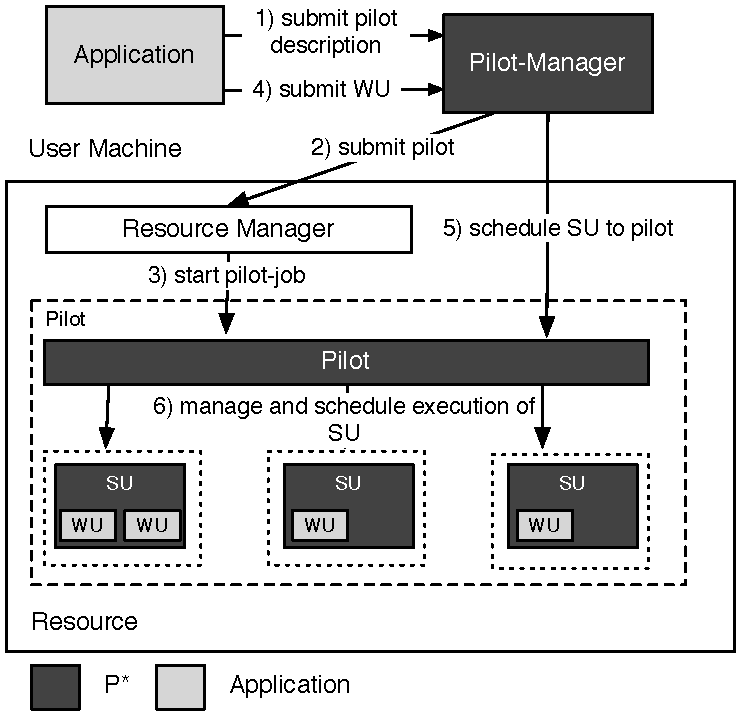
\includegraphics[width=0.48\textwidth]{figures/pstar_model_single.pdf}
    \caption{ \textbf{P* Model: Elements, Characteristics and
        Interactions:} The manager has two functions: it manages 1)
      Pilots (step 1-3) and 2) the execution of \cus. After a \cu is
      submitted to the manager, it transitions to an \su, which is
      scheduled to a \pilot by the PM. The \pilot then schedules the
      \su to an available resource.  }
    \label{fig:figures_pstar}
\end{figure}




%\input{sectionII_comments}

\noindent 
\subsection{Elements of the P* Model}


\noindent This sub-section defines the elements of the P* Model:


%\alnote{use pilot NOT pilot-job}
\noindent$\bullet$ \textbf{\pilot (Pilot-Compute):} The \pilot is the
  entity that actually gets submitted and scheduled on a resource.
% via the resource's RM system. 
  The PJ provides application (user)
  level control and management of the set of allocated resources.

  % and is responsible for the execution of \alwave{SUs/tasks}
  % onto the resource.

  % \alnote{\textbf{The RM assigns a slice of the Resource to the
  %     pilot -- that pilot then acts as RM for that resource slice.}
  %   I think simply equating a pilot with a RM is bit too
  %   simplistic. In a sense it is a application-level resource
  %   manger. Not sure what to do}

\noindent$\bullet$ \textbf{\computeunit  (\cu):} A \cu  encapsulates a 
  self-contained piece of work (a task) specified by the application that is
  submitted to the \pilotjob framework. There is no intrinsic notion
  of resource associated with a \cu.

\noindent$\bullet$ \textbf{Scheduling Unit (SU):} SUs are the units of 
  scheduling, internal to the P* Model, i.e., it is not known by or
  visible to an application. Once a \cu is
  under the control of the \pilotjob framework, it is assigned
  to an SU.
  % An SU is created after the submission of
  %   a \cu, i.\,e.\ once a \cu \ has been passed into the control of the
  %   pilot-job framework. 
%  \jhanote{Could we say: Once a \cu has been
%    passed into the control of the pilot-job framework, it is assigned
%    to an SU} \alnote{sounds good. done.}

\noindent$\bullet$ \textbf{Pilot-Manager (PM):} The PM is responsible for (i)
  orchestrating the interaction between the \pilots as well as the
  different components of the P* Model (\cus, \sus) and (ii) decisions
  related to internal resource assignment (once resources have been
  acquired by the \pilotjob).  For example, an SU can consists of one
  or more \cus. Further, \cus and \sus can be combined and aggregated;
  the PM determines how to group them, when \sus are scheduled and
  executed on a resource via the \pilot, as well as how many resources
  to assign to an SU.

% the different characteristics of the P* model. It
%   facilitates the coordination between the different P* elements,
%   i.\,e.\ the pilots, \cus and SUs. 
% A PM can e.\,g.\ manage solely one
%   or multiple pilots.

%   For example, the PM has the flexibility to combine and schedule \cus,
%   e.\,g.\ it can determine when a \cu is run and what as well as how
%   many resources it will receive.


% The application itself is not strictly part of the core P* Model.
% The term application generally refers to the upper layer of the
% stack.

An application kernel is the actual binary that gets executed.  The
application utilizes a PJ framework to execute multiple instances of
an application kernel (an ensemble) or alternatively instances of
multiple different application kernels (a workflow).  To execute an
application kernel, an application must define a \cu \ specifying the
application kernel as well as other parameters. This \cu \ is then
submitted to the PM (as an entry point to the
\pilotjob framework), where it transitions to an SU. The PM is then
responsible for scheduling the SU onto a \pilot and then onto a
physical resource.  As we will see in \S\ref{sec:pilot-job-frameworks}, 
the above elements can
be mapped to specific entities in many \pilotjobs in existence and
use; often more than one logical element may be rolled into a specific
entity in a \pilotjob.

% \textbf{Diane Definition of Terms: } The computation consists of
% many worker processes which communicate with one master process (the
% worker processes do not need to share the filesystem nor
% memory). The ensemble of computation is called a run and it consists
% of many tasks which may be executed in parallel. A task is defined
% as a set of parameters which are produced by the RunMaster (running
% on a master node) and consumed by the WorkerAgent (running on a
% worker node).
% 
% from 
% 
% DIANE assumes the master-worker computing model (Fig.
% 1). Client sends job parameters to the Planner which partitions
% the job into smaller tasks executed by the Workers. Integrator
% is responsible for merging the results of task execution and
% sending the final job outcome to the Client.


\subsection{Characteristics of P* Model}
\label{sec:p_star_elements}


%\jhanote{Why not have Binding as the first characteristics?}

% To understand % the degrees of freedom that any specific pilot-job
% % implementation must constraint as well as
% the functioning of
% pilot-jobs implementation, 
%These characteristics are integral components of the P* Model, in
% Further, these properties are important for the implementation of
% P*.  list several characteristics.
% The way the coordination between the different elements
% is handled is required to understand a PJ implementation.
 
We propose a set of fundamental properties/characteristics that
describe the interactions between the elements, and thus aid in the
description of P* Model.

% \alnote{ok} \jhanote{One strategy could be to not define the different
%   types, but just list/enumerate? Akin to Communication. i.e. explain
%   what coordination is for, what is being coordinated, how (the 3
%   types)}

\textbf{Coordination:} The coordination characteristics describe how
various elements of the P* Model, i.\,e.\ the PM, the \pilot, the \cus
and the SUs, interact. A common coordination pattern is master/worker
(M/W): the PM represents the master process that controls a set of
worker processes, the \pilots. The point of decision making is the
master process. In addition to the \emph{centralized} M/W, M/W can
also be deployed \emph{hierarchically}.  Alternatively, coordination
between the elements, in particular the \pilots, can be performed so as
to be \emph{decentralized}, i.\,e.\ without central decision making
point.

%\input{sectionIII-comments}

\textbf{Communication:} The communication characteristics describes the
mechanisms for data exchange between the elements of the P* Model:
e.\,g.\ messages (point-to-point, all-to-all, one-to-all, all-to-one,
or group-to-group), streams (potentially unicast or multicast),
publish/subscribe messaging or shared data spaces.
		
\textbf{Scheduling:} The scheduling characteristics describes the
process of mapping a SU to resources via a \pilot and potential
multiple levels of scheduling. Scheduling has a spatial component
(which SU is executed on which \pilot?) but also a temporal component
(when to bind?). The different scheduling decisions that need to be
made are representative of multi-level scheduling decisions that are
often required in distributed environments.  For example, when should
a SU be bound to a \pilot?  An SU can be bound to a \pilot either before
the \pilot has in turn been scheduled ({\it early} binding), whereas
{\it late} binding occurs if the SU is bound after the \pilot has been
scheduled.  In general, there are multiple-levels at which scheduling
decisions, i.e., resource selection and binding, are made.

The term {\it agent}, although not a part of the P* Model, finds
mention when discussing implementations. For the purposes of this
paper, an agent refers to a ``proxy process'' 
% that either % inside the % pilot-job framework
that has some decision making capability, and could aid the
implementation of one or more of the characteristics of the P* Model
-- coordination, communication, scheduling, within a \pilotjob
framework.  These agents can be used to enforce a set of
(user-defined) policies (e.g.  resource capabilities, data/compute
affinities, etc.) and heuristics.

\subsection{Putting it all together} 


Figure~\ref{fig:figures_pstar}
illustrates the interactions between the elements of the P* Model. First, the application specifies the capabilities of the
resources required using a \pilotjob description (step 1). The PM then
submits the necessary number of \pilots  to fulfill the
resource requirements of the application (step~2). Each \pilot is
queued at the resource manager, which is responsible for starting the
\pilot (step~3). There can be variations of this flow: while in the
described model, the application defines the required resources, the
PM could also decide based on the submitted \cu \ workload whether and
when it submits new \pilots.

%\jhanote{What about the Resource Manager? Is it part of the resource}

The application can submit \cus to the PM at any time (step~4). A
submitted \cu \ becomes an SU, i.\,e.\ the PM is now in control of
it. In the simplest case one \cu \ corresponds to one SU; however,
SUs can be combined and aggregated to optimize throughputs and
response times. Commonly, a hierarchical M/W model for coordination
is used internally: the PM uses M/W to coordinate a set of \pilots,
the \pilot itself functions as manager for the execution of the
assigned SUs.


Scheduling decisions can be made on multiple levels. The PM is responsible for
selecting a \pilot for an SU (step 5). A \pilot is bound to a physical resource
on which it is responsible for a particular resource set. Once a SU has been
scheduled to a \pilot, the \pilot decides when and on which part of the resource
an SU is executed.
% \jhanote{Isn't
%   the pilot already bound to a specific resource? Or isn't the pilot
%   bound to a resource and thereby the SU bound to a resource
%   indirectly, and not directly?}  \alnote{Yes, the pilot is bound to a
%   specific resource set, assigning a SU to a pilot means that it can
%   be executed somewhere on this resource set. The pilot decides on
%   which node a SU is run. There can be trivial cases, e.g. DIANE where
%   this decision making does not exist: 1 worker agent == 1 core == 1
%   task. Should we make this more explicit?} \jhanote{Yes -- we
%   could/should make more explicit the fact that pilot is already bound
%   to a resources and assigning a SU to a pilot means it can be
%   executed anywhere on this resource set.} \alnote{refined}
Further, the \pilot manages the subsequent execution of an SU (step~6).
There can be variations of this flow. 
% The above description presents a
% typical example of the inner working of a PJ framework, but alternative
% implementation of the P* characteristics are possible. 
PJ frameworks with decentralized decision making e.\,g.\ often utilize autonomic 
agents that accept respectively pull SUs according to a set of defined policies.


\begin{table*}[t]
 
 \centering
 \begin{tabular}{|p{3.1cm}|p{2.5cm}|p{2.0cm}|p{3.3cm}|p{3.5cm}|}
  \hline
  \textbf{P* Element}    &\textbf{BigJob} &\textbf{DIANE} &\textbf{Condor-G/Glide-in}     &\textbf{Swift/Coaster}  \\\hline
  Pilot-Manager          &BigJob Manager  & RunMaster     & condor\_master,\newline 
                                                            condor\_collector,\newline 
                                                            condor\_negotiator,\newline 
                                                            condor\_schedd                &Coaster Service         \\\hline
  \pilot                 &BigJob Agent    & Worker Agent  &condor\_master,\newline
                                                           condor\_startd                 &Coaster Worker          \\\hline
  \computeunit  \ (CU)   &Task            &Task           &Job                            &Application Interface\newline Function (Swift Script)\\\hline
  Scheduling Unit \ (SU) &Sub-Job         &Task           &Job                            &Job                     \\\hline
% Dynamic Resources &no/yes &yes (AgentFactories)\\
% \hline
 \end{tabular}
 \caption{\textbf{Mapping P* elements and PJ Frameworks:} While each PJ framework maintains its own vocabulary, each of the P* elements can be mapped to one (or more) components of the different PJ frameworks.
 } 
 \label{table:bigjob-saga-diane}
\end{table*}


\section{Pilot-API: A Uniform API to Heterogeneous PJ Frameworks}
\label{sec:pilot-api}

\section{Experiments and Results}
\label{sec:exp_res}

\section{P* as a Model for Pilot-Data}
\label{sec:pilot-data}

Many scientific applications have immense data requirements, which are
projected to increase dramatically in the near
future~\cite{hey2009}. The small genome alignment tool
scenario presented above e.\,g.\ operates on a input data set of
$>7$\,GB. While Pilot-Jobs efficiently support late-binding of
\computeunits and resources, the management of data in distributed
systems remains a challenge due to various reasons: (i) the placement
of data is often decoupled from the placement of Compute Units and
Pilots, i.\,e.\ the application must often manually stage in and out
its data using simple scripts;  (ii) heterogeneity, e.\,g.\ with
respect to storage, filesystem types and paths, often prohibits or at
least complicates late binding decisions; (iii) higher-level
abstraction that allow applications to specify their data dependencies
on an abstract, logical level (rather than on file basis) are not
available; (iv) due to lack of a common treatment for compute and
data, optimizations of data/compute placements are often not
possible. For example, in scenario (B3) and (B4) presented in
section~\ref{sec:fg-xsede-osg-egi}, even though the 50\,\% of the
input data set is shared for all \cus, the complete data is staged for
each \cu.

In addition, applications must cope with various other challenging,
data-related issues, e.\,g.\ varying data sources (such as sensors
and/or other application components), fluctuating data rates, transfer
failures, optimizations for different queries, data-/compute
co-location etc. While these issues can be in principal handled in an
application-specific way, the usage of higher-level abstractions, such
as a common \pilot-based abstraction for compute and data is
preferable.  

% Thus, having defined the P* model, we explore its extension to data.

This motivates an analogous abstraction that we call \emph{\pilotdata
  (PD)}. \jwave{PD provides late-binding capabilities for data by
  separating the allocation of physical storage and application-level
  data units.} Further, it provides an abstraction for expressing and
managing relationships between data units and/or compute units. These
relationships are referred to as \emph{affinities}.

% \jhanote{difficult to use affinity without defining it..}
% \alnote{tried to describe affinities a little bit better}

%\alnote{Extension vs. Application vs. Translation}
\subsubsection*{P* Model Elements for Data}

% A Pilot-Data Framework facilitates the late-binding between data units
% and physical storage resources, the so called pilot-stores.

The elements defined by P* (in section~\ref{sec:p_star_elements}) can
be extended by the following elements:

%\alnote{What is the role of SU in Data?}

\noindent$\bullet$
  \textbf{\pilot (Pilot-Data):} A \pilotdata (\pd) functions as a 
	placeholder object that reserves the space
	for data units. PD facilitates the late-binding of data and resource and is
	equivalent to the \pilot in the compute model.

\noindent$\bullet$
  \textbf{Data Unit (DU):} DU is the base unit of data assigned by
  the application,  e.\,g.\ a data file or chunk. Multiple DUs can be aggregated 
   within a Data Unit Set.

% \noindent$\bullet$ \textbf{Pilot-Data (PD):} PD allows the logical grouping of DUs
%   and the expression of data-data affinities. This collection of files
%   can be associated with an extensible set of properties. One of these
%   properties is affinity. 

\noindent$\bullet$
  \textbf{Scheduling Unit (SU):} is an internal unit of scheduling (as in 
  the compute case). The Pilot framework can aggregate or split DUs into one 
  or more SUs.

\noindent$\bullet$ 
  The \textbf{Pilot-Manager (PM)} is the same as in the compute model and
  implements the different characteristics of the P* Model. It is responsible for
  managing \dus and \sus. Data is submitted to the framework via the PM. The PM
  which is responsible for mapping \dus to \sus and for conducting decision 
  regarding resource assignments. \sus are placed on physical resources via the \pilot.

Note, each element can be mapped to an element in the P* Model by
symmetry, e.\,g., a DU correspond to a \cu  in the original P* Model; 
a PD is a placeholder reserving a certain amount of storage on a physical 
resource and corresponds to the \pilot in the P* Model.

% \jhanote{PJ Model is confusing. Either it is P Model or PJ
%   Framework} \alnote{ok}

% A particular critical requirement for data-intensive application, is
% the management of affinity between DUs and also between \cus and
% DUs. Thus, Pilot-Data introduces the PD container object for
% expressing relationships between DUs. A PD corresponds to an SU in
% the \jwave{PJ model}, i.\,e.\ it is used as scheduling unit for
% internal optimizations, e.\,g.\ the grouping of DUs. Having
% instantiated a PD, it can be assigned to a PS via the PD manager. A
% PS is a placeholder reserving a certain amount of storage, i.\,e.\
% it corresponds to a pilot in the pilot-job model. By associating a
% PD to a PS the data is actually moved to the physical location
% associated with the PS. The PD manager facilitates the creation of
% PSs, schedules data movements (with respect to specified affinities)
% and manages data accesses.

\subsubsection*{P* Model Characteristics for Data}

While the extended P* Model introduces new elements, the
characteristics however, remain the same to a great extent. The
coordination characteristic describes how the elements of PD interact,
e.\,g.\ utilizing the M/W model; the communication characteristic can
be applied similarly. The scheduling characteristics must be extended
to not only meet compute requirements, but also to support common data
access patterns. \jhanote{Propose comment out due to space
  restrictions: The scheduling component particularly needs to
  consider affinities, i.\,e.\ user-defined relationships between \cus
  and/or \dus. Data-data affinities e.\,g.\ exist if different \dus
  must be present at the same compute element; data-compute affinities
  arise if data and compute must be co-located for a computation, but
  their current location is different.} Data and compute placement
decisions are made by the scheduler based on defined policies,
affinities \& dynamic resource information.


\subsubsection*{Pilot-API for Data} 

Analogous to the Pilot-API for Compute, the Pilot Data API~\cite{pilot_api} 
defines the \texttt{PilotDataService} entity as an abstraction for creating and
managing pools of storage. A \texttt{PilotData} instance represents the actual
physical storage space. The \texttt{ComputeDataService} entity
functions as an application-level scheduler, which accepts both
\texttt{Compute\-Units} and \texttt{DataUnits}. It resolves necessary
dependencies (e.g. data/data or data/computer affinities), and is
responsible for managing the execution of \dus and \cus.



\section{Discussion and Future Work}
\label{sec:discussion-future-work}

The primary intellectual contribution of this work has been the
development of the P* Model, the mapping of P* elements to PJ
frameworks such as DIANE and Condor-G/Glide-in and the design and
development of the Pilot-API -- that reflects the P* elements and
characteristics.
 
The P* Model provides a common abstract model for describing and
characterizing Pilot-abstractions.  We validate the P* Model by
demonstrating that the most widely used PJ frameworks, viz., DIANE and
Condor-G/Glide-in can be compared, contrasted and analyzed using this
analytical framework.  Furthermore we demonstrate the use of the
Pilot-API -- which provides a common access layer to different PJ
frameworks, with multiple PJ frameworks over distributed production
cyberinfrastructure, such as XSEDE, OSG, EGI and FutureGrid. The
Pilot-API also enables the concurrent use of multiple PJ frameworks,
thus providing interoperability and extensibility.  Although the aim
of our experiments is the demonstration of the interoperable use of
hitherto distinct and disjoint \pilotjobs, in the process we highlight
the performance advantages that can emanate from the ability to
seamlessly distribute (I/O intensive) workloads in a scalable manner.


% \section*{Acknowledgements}
% This work is funded by NSF CHE-1125332 (Cyber-enabled Discovery and
% Innovation), HPCOPS NSF-OCI 0710874 award, NSF-ExTENCI (OCI-1007115)
% and NIH Grant Number P20RR016456 from the NIH National Center For
% Research Resources. Important funding for SAGA has been provided by
% the UK EPSRC grant number GR/D0766171/1 (via OMII-UK) and the
% Cybertools project (PI Jha) NSF/LEQSF
% (2007-10)-CyberRII-01. SJ acknowledges the e-Science Institute,
% Edinburgh for supporting the research theme. ``Distributed Programming
% Abstractions'' \& 3DPAS. MS is sponsored by the program of BiG Grid,
% the Dutch e-Science Grid, which is financially supported by the
% Netherlands Organisation for Scientific Research, NWO. SJ acknowledges
% useful related discussions with Jon Weissman (Minnesota) and Dan Katz
% (Chicago). We thank J Kim (CCT) for assistance with BFAST.  This work
% has also been made possible thanks to computer resources provided by
% TeraGrid TRAC award TG-MCB090174 (Jha) and BiG Grid.  This document
% was developed with support from the US NSF under Grant No. 0910812 to
% Indiana University for ``FutureGrid: An Experimental, High-Performance
% Grid Test-bed''.

% %\bibliographystyle{plain}
% %\bibliographystyle{IEEEtranS}
% \bibliographystyle{IEEEtran}
% %\bibliography{pilotjob,saga,saga-related}
% \bibliography{pstar-hpdc2012}

\end{document}
